% Sketch of a jet (left: AK4 jet with displaced secondary vertex; right: boosted AK8 jet
% containing two subjets). Compile with: pdflatex jets_sketch.tex
\documentclass[tikz,border=4pt]{standalone}
\usepackage{amsmath}
\usetikzlibrary{arrows.meta,calc,decorations.pathreplacing}

\definecolor{cmsblue}{RGB}{31,90,166}
\definecolor{cmsred}{RGB}{200,40,40}
\definecolor{cmsgray}{RGB}{120,120,120}
\definecolor{jetgreen}{RGB}{70,140,90}
\definecolor{jetviolet}{RGB}{95,85,160}

\begin{document}
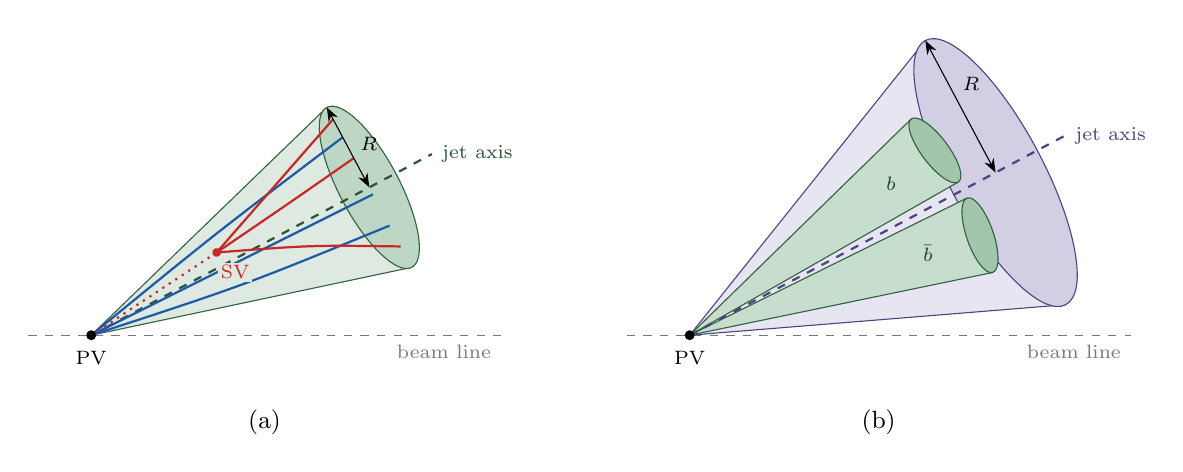
\begin{tikzpicture}[>={Stealth[length=5pt]}, font=\small]

% ------------------------------------------------------------------
% (a) AK4 jet with a displaced secondary vertex
% ------------------------------------------------------------------
\begin{scope}
  % beam line and primary vertex
  \draw[cmsgray, dashed] (-0.8,0) -- (5.2,0);
  \node[cmsgray, font=\scriptsize, anchor=north east] at (5.2,0) {beam line};
  \begin{scope}[rotate=28]
    % cone
    \fill[jetgreen!18] (0,0) -- (4,1.15) arc[start angle=90, end angle=-90, x radius=0.38, y radius=1.15] -- cycle;
    \draw[jetgreen!70!black] (0,0) -- (4,1.15);
    \draw[jetgreen!70!black] (0,0) -- (4,-1.15);
    \fill[jetgreen!35] (4,0) ellipse[x radius=0.38, y radius=1.15];
    \draw[jetgreen!70!black] (4,0) ellipse[x radius=0.38, y radius=1.15];
    % jet axis
    \draw[jetgreen!60!black, dashed, thick] (0,0) -- (4.9,0) node[anchor=west, font=\scriptsize] {jet axis};
    % prompt tracks from the primary vertex
    \draw[cmsblue, thick] (0,0) .. controls (2,0.4) .. (4,0.72);
    \draw[cmsblue, thick] (0,0) .. controls (2,-0.35) .. (4,-0.55);
    \draw[cmsblue, thick] (0,0) .. controls (2,-0.05) .. (4,-0.1);
    % displaced secondary vertex and its tracks
    \coordinate (SV) at (1.9,0.18);
    \draw[cmsred, thick] (SV) .. controls (3.0,0.6) .. (4,0.98);
    \draw[cmsred, thick] (SV) .. controls (3.0,-0.3) .. (4,-0.85);
    \draw[cmsred, thick] (SV) .. controls (3.0,0.3) .. (4,0.42);
    \draw[cmsred, dotted, thick] (0,0) -- (SV);
    \fill[cmsred] (SV) circle (1.6pt);
    \node[cmsred, font=\scriptsize, anchor=north, fill=jetgreen!18, inner sep=1pt] at ($(SV)+(0.15,-0.22)$) {SV};
    % cone radius
    \draw[<->, black] (4,0) -- (4,1.15);
    \node[anchor=west, font=\scriptsize] at (4.05,0.6) {$R$};
  \end{scope}
  \fill (0,0) circle (1.8pt);
  \node[anchor=north, font=\scriptsize] at (0,-0.08) {PV};
  \node[font=\small] at (2.2,-1.1) {(a)};
\end{scope}

% ------------------------------------------------------------------
% (b) boosted AK8 jet containing two subjets
% ------------------------------------------------------------------
\begin{scope}[xshift=7.6cm]
  \draw[cmsgray, dashed] (-0.8,0) -- (5.6,0);
  \node[cmsgray, font=\scriptsize, anchor=north east] at (5.6,0) {beam line};
  \begin{scope}[rotate=28]
    % large-radius cone
    \fill[jetviolet!15] (0,0) -- (4.4,1.9) arc[start angle=90, end angle=-90, x radius=0.6, y radius=1.9] -- cycle;
    \draw[jetviolet!80!black] (0,0) -- (4.4,1.9);
    \draw[jetviolet!80!black] (0,0) -- (4.4,-1.9);
    \fill[jetviolet!28] (4.4,0) ellipse[x radius=0.6, y radius=1.9];
    \draw[jetviolet!80!black] (4.4,0) ellipse[x radius=0.6, y radius=1.9];
    % two subjets
    \foreach \ang/\lab in {9/b, -9/\bar{b}} {
      \begin{scope}[rotate=\ang]
        \fill[jetgreen!30] (0,0) -- (3.9,0.5) arc[start angle=90, end angle=-90, x radius=0.17, y radius=0.5] -- cycle;
        \draw[jetgreen!70!black] (0,0) -- (3.9,0.5);
        \draw[jetgreen!70!black] (0,0) -- (3.9,-0.5);
        \fill[jetgreen!50] (3.9,0) ellipse[x radius=0.17, y radius=0.5];
        \draw[jetgreen!70!black] (3.9,0) ellipse[x radius=0.17, y radius=0.5];
        \node[jetgreen!50!black, font=\scriptsize] at (3.2,0) {$\lab$};
      \end{scope}
    }
    % large-jet axis
    \draw[jetviolet!80!black, dashed, thick] (0,0) -- (5.4,0) node[anchor=west, font=\scriptsize] {jet axis};
    % cone radius
    \draw[<->, black] (4.4,0) -- (4.4,1.9);
    \node[anchor=west, font=\scriptsize] at (4.45,1.25) {$R$};
  \end{scope}
  \fill (0,0) circle (1.8pt);
  \node[anchor=north, font=\scriptsize] at (0,-0.08) {PV};
  \node[font=\small] at (2.4,-1.1) {(b)};
\end{scope}

\end{tikzpicture}
\end{document}
